\section{Experiments}
\label{sec:experiments}

We study \tvc{} in two settings. In a multi-agent bandit, where agents search arms of unknown value on behalf of a group. In a congestion setting built on a multi-agent pathfinding (MAPF) benchmark \citep{skrynnik2025pogema}, robots can post fake jams to clear their own routes. 

\subsection{Experiment 1: Multi-agent Bandit} \label{subsec:experiment1}

\paragraph{Setup.}
$N=10$ agents search $K=50$ arms whose values are drawn i.i.d.\ from a lognormal distribution, in episodes of $T=100$ rounds, and each agent starts knowing one random arm. In each round a free agent either explores a random arm, at a cost of $0.5\vbar$, or exploits its best known arm. An explorer may post a claim about its find: silence, or the true value scaled by $\times1$ (truthful), $\times1.1$, $\times1.5$ or $\times2$. Free agents that did not explore follow the claim that beats their own best and stay committed for $L=3$ rounds. We use two kinds of receiver: naive receivers take a claim at face value, and calibrated receivers learn, for each sender, how far its claims exceed the truth, from the claims they have followed, with learning rate $0.3$. Explore and report decisions are learned by tabular REINFORCE (learning rate $0.1$, discount $0.9$, a running baseline per state), with the agent's own best and the value of its find as states.

\paragraph{Credit designs.}
We compare no credit, popularity credit ($2\vbar$ per follower), accuracy credit (the follower's signed gain), \tvc{} ($\tau=0.05$, $\Bbar=8$, $\eta=2$, $p=0.2$, $\varphi=8$, $w=0.05$), a shared return (every agent receives the group's mean payoff), credit for keeping exploring (a flat $3\vbar$ per exploration, matched to \tvc{}'s spend), a lying cost alone (audited false claims fined $\varphi$, nothing else given) and popularity credit with that fine. Reputation alone is no credit with calibrated receivers.

\paragraph{Metrics.}
Inflation (share of reports that are exaggerated), report rate (reports per exploration), misled follows (follows that lead to a worse arm), welfare (own payoff per round, in units of $\vbar$) and exploration rate. We report the mean over the last 100 of 1000 episodes with 95\% confidence intervals over 32 independent runs.

\paragraph{Results.}
\Cref{tab:bandit} compares the credit designs. Credit for being relied on breeds hype. With naive receivers, popularity credit raises inflation from 75.1\% (no credit) to 94.0\% and the share of misled follows from 25.5\% to 43.5\%. Accuracy credit does not remove it (68.9\% with naive and 85.1\% with calibrated receivers). \tvc{} brings inflation down to 0.3\% with naive and 0.4\% with calibrated receivers, raises the report rate to 99.6\%, and cuts misled follows to 0.2\%. A lying cost alone also removes most inflation (3.4\%), but half of the explorers choose to silent (report rate 50.0\%), and it has the lowest welfare (3.18 against 3.49 with no credit). Popularity credit with the same fine still has 38.4\% inflation. In welfare, \tvc{} (4.03) matches popularity credit (4.04) and exceeds no credit (3.49). The highest welfare comes from keeping exploring (4.28), which raises the exploration rate to 15.0\% against 3.0\% for \tvc{} but leaves inflation at 74.7\%. The shared return also raises exploration (23.3\%) but reaches the same welfare as \tvc{} (4.06) with 71.9\% inflation. \tvc{} therefore makes reports honest at no cost in welfare, but it does not by itself increase exploration. Calibrated receivers lower the cost of hype, as the conditions in \cref{sec:when} predict. With no credit they cut misled follows from 25.5\% to 7.6\%, and under popularity credit to 0.9\%, so popularity credit reaches the welfare of \tvc{} (4.02 against 3.96, within the intervals) at 92.2\% inflation.

% Multi-agent bandit, 1000 episodes, 32 runs, last 100 episodes (source: logs/bandit_run3.log, python -m tvc.bandit 1000).
% ICML: table captions go ABOVE the table.
\begin{table*}[t]
  \caption{Multi-agent bandit: credit designs compared (mean $\pm$ 95\% CI over 32 runs, last 100 of 1000 episodes). Inflation is the percentage of reports that are exaggerated, report is the percentage of explorations that are reported, misled is the percentage of follows that lead to a worse arm, and explore is the percentage of agent-rounds spent exploring. Welfare is the mean own payoff per agent per round, in units of the mean arm value. With calibrated receivers, \emph{None} is reputation only. \emph{Keeping exploring} gives a flat $3\vbar$ per exploration, \emph{Lying cost alone} fines audited false claims and gives nothing else, and \emph{Shared return} gives every agent the group mean payoff.}
  \label{tab:bandit}
  \centering
  \small
  \setlength{\tabcolsep}{4pt}
  \begin{tabular}{lccccc}
    \toprule
    Credit design & Inflation (\%)  & Report (\%)  & Misled (\%)  & Welfare ($\vbar$)  & Explore (\%) \\
    \midrule
    \multicolumn{6}{l}{\emph{Naive receivers}} \\
    None & $75.1 \pm 0.4$ & $80.2 \pm 0.3$ & $25.5 \pm 1.0$ & $3.486 \pm 0.104$ & $2.7 \pm 0.2$ \\
    Popularity & $94.0 \pm 0.5$ & $94.8 \pm 0.4$ & $43.5 \pm 1.1$ & $4.036 \pm 0.054$ & $4.5 \pm 0.2$ \\
    Accuracy & $68.9 \pm 2.4$ & $89.8 \pm 0.4$ & $13.7 \pm 1.2$ & $3.867 \pm 0.095$ & $2.9 \pm 0.2$ \\
    Shared return & $71.9 \pm 5.4$ & $80.1 \pm 4.7$ & $32.7 \pm 4.8$ & $4.055 \pm 0.145$ & $\mathbf{23.3 \pm 3.0}$ \\
    Keeping exploring & $74.7 \pm 1.1$ & $79.1 \pm 1.2$ & $41.3 \pm 1.8$ & $\mathbf{4.280 \pm 0.083}$ & $15.0 \pm 2.5$ \\
    Lying cost alone & $3.4 \pm 0.7$ & $50.0 \pm 2.9$ & $1.4 \pm 0.3$ & $3.177 \pm 0.114$ & $2.4 \pm 0.2$ \\
    Popularity + fine & $38.4 \pm 1.6$ & $85.0 \pm 2.4$ & $34.4 \pm 1.6$ & $3.859 \pm 0.070$ & $3.4 \pm 0.2$ \\
    \textbf{TVC} & $\mathbf{0.3 \pm 0.1}$ & $\mathbf{99.6 \pm 0.1}$ & $\mathbf{0.2 \pm 0.1}$ & $4.028 \pm 0.079$ & $3.0 \pm 0.2$ \\
    \midrule
    \multicolumn{6}{l}{\emph{Calibrated receivers (per-sender decoding)}} \\
    None & $75.1 \pm 0.5$ & $80.1 \pm 0.4$ & $7.6 \pm 0.5$ & $3.528 \pm 0.126$ & $2.5 \pm 0.3$ \\
    Popularity & $92.2 \pm 0.5$ & $93.4 \pm 0.5$ & $0.9 \pm 0.4$ & $4.023 \pm 0.078$ & $3.2 \pm 0.2$ \\
    Accuracy & $85.1 \pm 1.3$ & $90.6 \pm 0.4$ & $3.3 \pm 0.5$ & $3.993 \pm 0.097$ & $3.1 \pm 0.3$ \\
    Shared return & $68.0 \pm 6.8$ & $83.6 \pm 3.4$ & $3.3 \pm 0.7$ & $4.118 \pm 0.159$ & $\mathbf{23.7 \pm 3.6}$ \\
    Keeping exploring & $74.8 \pm 1.2$ & $79.2 \pm 1.1$ & $9.1 \pm 0.6$ & $\mathbf{4.358 \pm 0.079}$ & $15.1 \pm 2.6$ \\
    Lying cost alone & $3.5 \pm 0.7$ & $50.4 \pm 3.6$ & $1.3 \pm 0.2$ & $3.045 \pm 0.128$ & $2.2 \pm 0.3$ \\
    Popularity + fine & $33.4 \pm 2.3$ & $85.4 \pm 2.5$ & $2.5 \pm 0.4$ & $3.877 \pm 0.094$ & $2.5 \pm 0.2$ \\
    \textbf{TVC} & $\mathbf{0.4 \pm 0.1}$ & $\mathbf{99.6 \pm 0.2}$ & $\mathbf{0.2 \pm 0.1}$ & $3.963 \pm 0.081$ & $2.9 \pm 0.2$ \\
    \bottomrule
  \end{tabular}
\end{table*}


\subsection{Experiment 2: MAPF with fake jams} \label{subsec:experiment2}

\paragraph{Setup.}
We use POGEMA's lifelong pathfinding task \citep{skrynnik2025pogema} with soft collisions on a $3\times3$ layout of $5\times5$ rooms joined by 1-cell doorways, with 12 robots, observation radius $3$ and $256$ steps. Robots move by greedy descent on a distance map, so the only learned decision is whether to post a claim that a doorway they can see is jammed. We define the ground truth that a doorway is jammed when at least $3$ robots are within $2$ walking steps of it. Receivers that believe a claim avoid that doorway for $20$ steps, and a claim expires after $20$ steps. A claim is checked by a robot that passes the doorway, or by an audit. Naive receivers take claims at face value, and sceptical receivers learn per-sender trust from the checks they see (learning rate $0.3$).

\paragraph{Mixed motive.}
A robot's reward is $(1-\lambda)$ times its own deliveries plus $\lambda$ times the others' mean deliveries, minus a cost per claim posted, plus credit. A lie, a fake jam on its own route, gains the liar when believers leave that route and costs the others their detours. The per-believer gain, harm and benefit that enter the learning signal are calibrated from short runs with hand-set policies, and the temptation is therefore a modelling choice, not an emergent property. Claim policies are learned by tabular REINFORCE.

\paragraph{Credit designs.}
No credit, popularity credit ($1$ per believer), accuracy credit (the steps a believer saves, negative for a fake jam), \tvc{} ($\tau=0.05$, $\Bbar=8$, $\eta=2$, $p=0.2$, $\varphi=15$), reputation (no credit, sceptical receivers) and a shared return ($\lambda=(N-1)/N$).

\paragraph{Metrics.}
We report the lie rate (the share of opportunities on which a robot posts a fake jam on its own route), the useful-report rate (the share of real jams elsewhere that it reports), POGEMA's throughput (deliveries per step, summed over the 12 robots) and the credit given, as the mean over the last 50 of 150 episodes, with 95\% confidence intervals over 10 seeds.

\paragraph{Questions.}
We ask  questions. Does lying harm the group, so that honest reports are worth rewarding? Does \tvc{} remove lying and raise throughput compared with the other credit designs? Does it do so at every prosocial weight?.

\paragraph{Lying harms the group.}
We first check that lying is costly for the group, because only then is it worth rewarding honest reports. We fix the claim policies instead of learning them. The first $k$ of the 12 robots post a fake jam whenever a doorway on their own route is free, the others report real jams, and no credit is given. We run 10 batches of 20 episodes for each $k$, with 95\% confidence intervals over batches. With naive receivers, group deliveries per robot per episode fall from 5.8 with no liars to 1.9 with 12 (\cref{fig:hype}), and the share of detours that were for fake jams rises from 0.31 at $k=1$ to 0.95 at $k=12$. One liar gains 3.5 deliveries over its honest peers while the others lose 0.5, so a single lie mostly moves deliveries from the others to the liar, and the group loses clearly once several robots lie. Sceptical receivers, which learn a trust for each sender from the checks they see, soften this: the group falls to 3.7 at $k=12$, and a liar's advantage at $k=1$ falls from 3.5 to 1.6. A lying robot still delivers more than an honest one at every $k<12$. Each episode starts with full trust, so this understates what trust learned over many episodes would do.

\begin{figure*}[t]
  \centering
  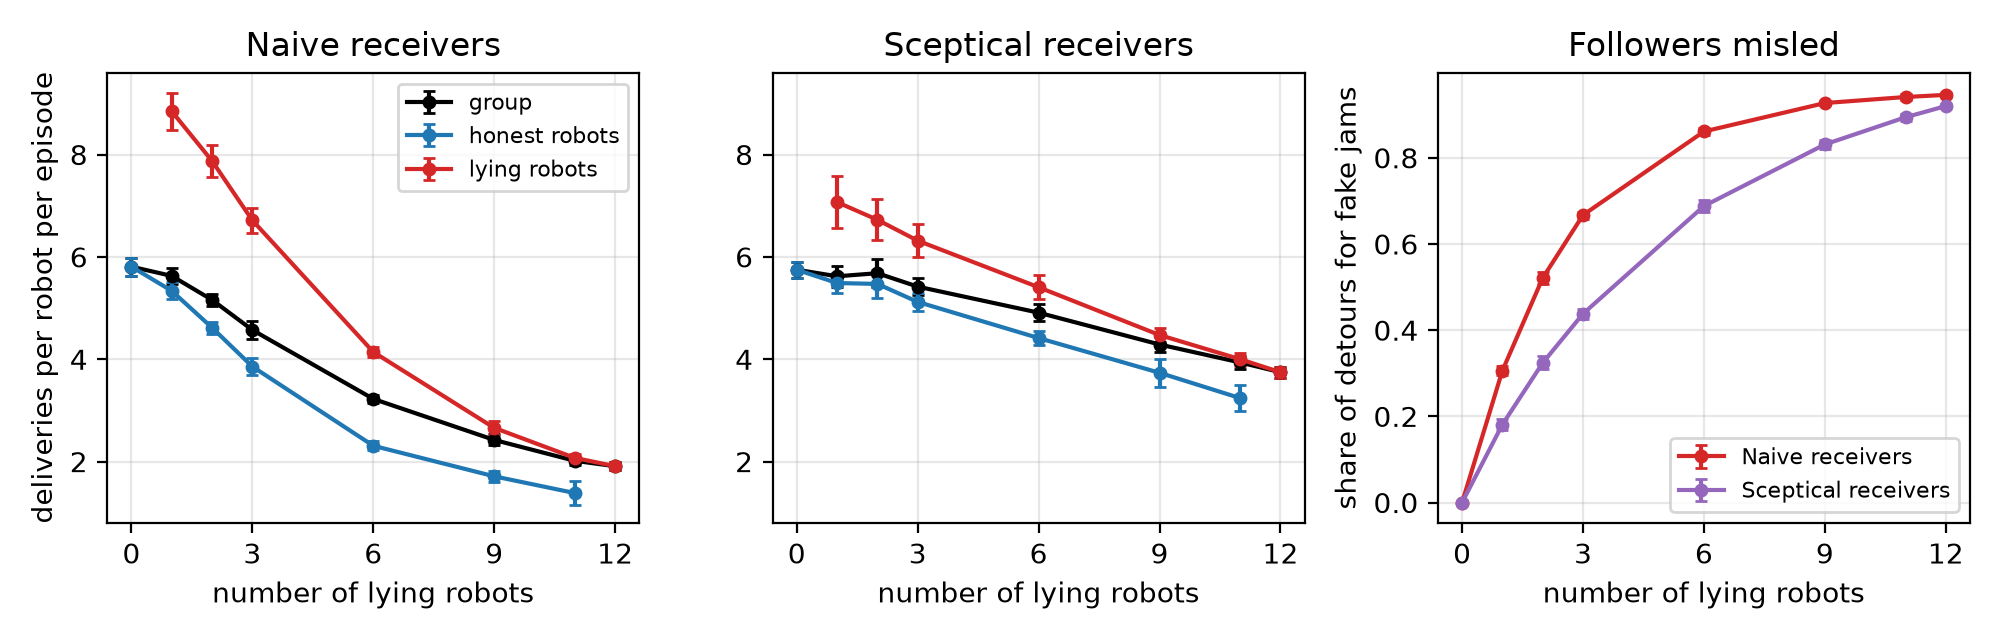
\includegraphics[width=\textwidth]{figures/fake_jams_hype_compare.png}
  \caption{Lying harms the group in the congestion setting. The first $k$ of 12 robots post fake jams and the rest report real jams, with fixed policies and no credit (10 batches of 20 episodes, 95\% CIs). Left and middle: deliveries per robot per episode for the group, the honest robots and the lying robots, with naive and with sceptical receivers. Right: share of detours that were for fake jams.}
  \label{fig:hype}
\end{figure*}

\paragraph{\tvc{} removes lying and raises throughput.}
\Cref{tab:pogema} gives the lifelong comparison at $\lambda=0$. Without credit, selfish robots post a fake jam on 99.2\% of their opportunities and report 44.7\% of the real jams elsewhere. Popularity credit leaves the lie rate at 99.9\% and raises useful reports to 94.6\%, but throughput falls from 0.080 to 0.037, as in the hype sweep, where throughput falls as more robots lie (\cref{fig:hype}). \tvc{} cuts the lie rate to 0.2\%, raises useful reports to 98.8\%, and raises throughput to 0.266, 3.3 times that of no credit and 7.2 times that of popularity credit.
% Ratios below are from logs/fake_jams_envs.md (3-decimal rounding), so they are approximate.
The other designs fall between these. Reputation alone, that is sceptical receivers with no credit, keeps the lie rate at 80.1\% and reaches only about 1.5 times the throughput of no credit. Accuracy credit removes lying (0.1\%) by silencing the robots, with 1.2\% useful reports, and its throughput is below that of no credit (about 0.75 times). A shared return with $\lambda=(N-1)/N$ is the closest competitor: it cuts lying to 6.3\% and reaches about 3.1 times the throughput of no credit, but it needs every robot to weigh the others' deliveries as much as its own, which \tvc{} does not.

% POGEMA lifelong MAPF, lambda = 0, 10 seeds (source: logs/fake_jams_pogema.md).
% ICML: table captions go ABOVE the table.
\begin{table}[t]
  \caption{POGEMA lifelong MAPF ($\lambda=0$, 10 seeds, mean $\pm$ 95\% CI). Lie rate is the percentage of opportunities on which a robot posts a fake jam on its own route, useful is the percentage of real jams elsewhere that it reports, and throughput is POGEMA's \texttt{avg\_throughput}, the deliveries per step summed over the 12 robots.}
  \label{tab:pogema}
  \centering
  \small
  \setlength{\tabcolsep}{3pt}
  \begin{tabular}{lccc}
    \toprule
    Rule & Lie rate (\%)  & Useful (\%)  & Throughput  \\
    \midrule
    None       & $99.2 \pm 0.0$ & $44.7 \pm 1.5$ & $0.080 \pm 0.002$ \\
    Popularity & $99.9 \pm 0.0$ & $94.6 \pm 0.8$ & $0.037 \pm 0.001$ \\
    \textbf{TVC} & $\mathbf{0.2 \pm 0.1}$ & $\mathbf{98.8 \pm 0.7}$ & $\mathbf{0.266 \pm 0.007}$ \\
    \bottomrule
  \end{tabular}
\end{table}


\paragraph{\tvc{} holds at every prosocial weight.}
Across the prosocial weight $\lambda$ (\cref{fig:lam}), popularity credit keeps the lie rate at 99.8--99.9\% and throughput at 0.003, and \tvc{} holds the lie rate at 0.2\% or less at every $\lambda$, with throughput 0.022--0.023. With no credit, lying is 99.2\% at $\lambda=0$ and still 91.9\% at $\lambda=0.75$, and falls to 2.5\% only at $\lambda=1$, where throughput rises to 0.021. This agrees with the calibrated threshold, $\lambda\approx0.93$, below which a lie is profitable without credit.

\begin{figure}[t]
  \centering
  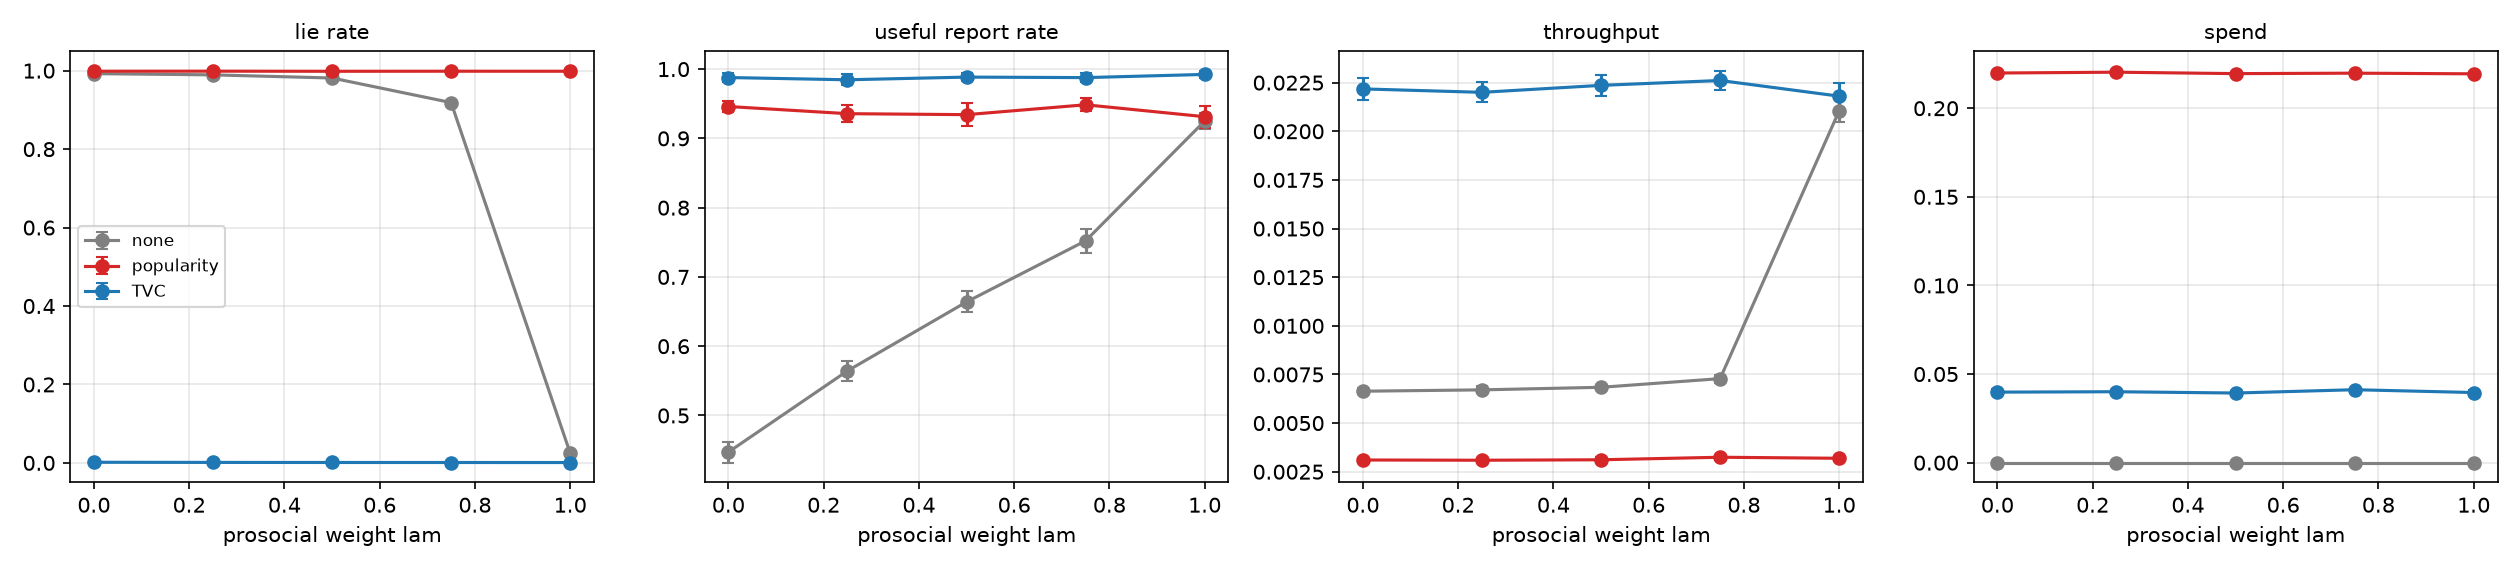
\includegraphics[width=\linewidth]{figures/fake_jams_lam.png}
  \caption{Learned behaviour by credit rule and prosocial weight $\lambda$ (10 seeds, 95\% CIs).}
  \label{fig:lam}
\end{figure}

% \paragraph{The fine follows the theory.}
% The fine sweep (\cref{fig:fine}, $\lambda=0$) brackets the calibrated threshold $\philo=2.25$. Lying is 99.3\% with no fine and 98.3\% at $0.5\philo$, falls to 62.4\% at $\philo$ and to 0.9\% at $2\philo$, so it collapses between $\philo$ and $2\philo$, within a factor of two of the theory. \Cref{app:ablation} also shows that removing the audits or the fine brings lying back, that the bonus is not needed in this setting, and that \tvc{} raises throughput only when receivers act on claims.

% \begin{figure}[t]
%   \centering
%   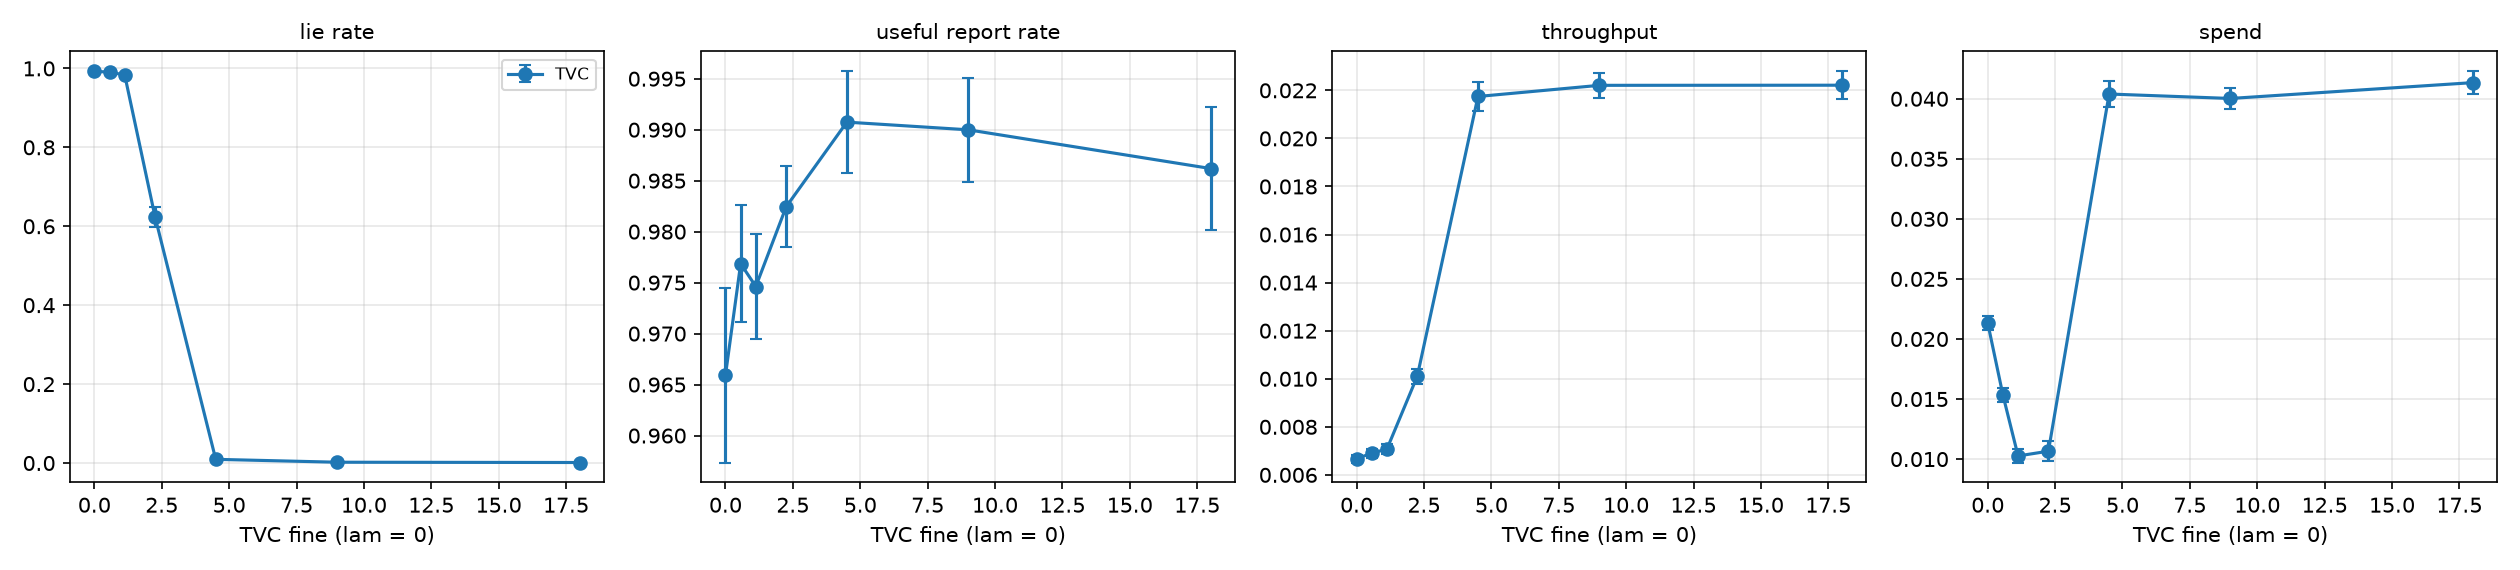
\includegraphics[width=\linewidth]{figures/fake_jams_fine.png}
%   \caption{TVC fine sweep at $\lambda=0$. Lying collapses between $\philo$ and $2\philo$ (10 seeds, 95\% CIs).}
%   \label{fig:fine}
% \end{figure}

% \todo{Scaling (agents, map size).}
